\section{Aufgabe 1}
\begin{center}
\begin{tabular}{c|c|c|c}
\(I_B\) in \(\mu A\) & \(I_C\) in \(mA\) & \(U_{BE}\) in \(V\) & \(U_{CE}\) in \(V\) \\ \hline
\(29.9\) & \(3.83\) & \(0.706\) & \(1.218\) \\ 
\(29.9\) & \(3.86\) & \(0.706\) & \(2.015\) \\ 
\(29.9\) & \(3.89\) & \(0.705\) & \(3.005\) \\ 
\(30.2\) & \(3.73\) & \(0.697\) & \(4.086\) \\ 
\(30.7\) & \(3.53\) & \(0.685\) & \(5.005\) \\ 
\(31.0\) & \(3.51\) & \(0.557\) & \(6.031\) \\ 
\(36.2\) & \(3.16\) & \(0.557\) & \(6.96\) \\ 
\(36.0\) & \(3.21\) & \(0.542\) & \(8.02\) \\ 
\(38.0\) & \(3.16\) & \(0.492\) & \(9.05\) \\ 
\(39.5\) & \(3.14\) & \(0.445\) & \(10.04\) \\ 
\(41.4\) & \(3.15\) & \(0.390\) & \(11.01\) \\ 
\(34.9\) & \(3.15\) & \(0.352\) & \(12.04\)
\end{tabular}
\captionof{table}{Rohmesswerte bei \(I_B \approx 30 \mu A\)}

\begin{tabular}{c|c|c|c}
\(I_B\) in \(\mu A\) & \(I_C\) in \(mA\) & \(U_{BE}\) in \(V\) & \(U_{CE}\) in \(V\) \\ \hline
\(61.4\) & \(9.65\) & \(0.726\) & \(1.157\) \\ 
\(64.5\) & \(7.52\) & \(0.688\) & \(2.019\) \\ 
\(67.6\) & \(7.4\) & \(0.652\) & \(3.051\) \\ 
\(61.4\) & \(10.73\) & \(0.725\) & \(3.973\) \\ 
\(61.8\) & \(10.97\) & \(0.721\) & \(5.011\) \\ 
\(61.9\) & \(11.12\) & \(0.718\) & \(6.007\) \\ 
\(62.1\) & \(11.26\) & \(0.716\) & \(6.96\) \\ 
\(62.3\) & \(11.46\) & \(0.712\) & \(8.09\) \\ 
\(62.7\) & \(11.64\) & \(0.71\) & \(8.98\) \\ 
\(62.9\) & \(11.86\) & \(0.705\) & \(10.01\) \\ 
\(63.1\) & \(12.04\) & \(0.702\) & \(11.02\) \\ 
\(63.5\) & \(12.17\) & \(0.702\) & \(12.04\)
\end{tabular}
\captionof{table}{Rohmesswerte bei \(I_B \approx 60 \mu A\)}

\begin{tabular}{c|c|c|c}
\(I_B\) in \(\mu A\) & \(I_C\) in \(mA\) & \(U_{BE}\) in \(V\) & \(U_{CE}\) in \(V\) \\ \hline
\( 88.4\) & \(15\) & \(0.738\) & \(1.1\) \\ 
\(88.4\) & \(14.94\) & \(0.741\) & \(2.097\) \\ 
\(88.4\) & \(15.03\) & \(0.741\) & \(2.967\) \\ 
\(88.8\) & \(15.26\) & \(0.739\) & \(3.945\) \\ 
\(89.9\) & \(14.65\) & \(0.731\) & \(5.02\) \\ 
\(93.3\) & \(11.91\) & \(0.7\) & \(6.643\) \\ 
\(95.3\) & \(11.72\) & \(0.688\) & \(7.03\) \\ 
\(98.3\) & \(10.58\) & \(0.652\) & \(8.16\) \\ 
\(99.9\) & \(10.5\) & \(0.643\) & \(9.06\) \\ 
\(102.0\) & \(10.51\) & \(0.627\) & \(10.01\) \\ 
\(105.0\) & \(10.55\) & \(0.601\) & \(11.06\) \\ 
\(105.5\) & \(10.66\) & \(0.59\) & \(12.00 \)
\end{tabular}
\captionof{table}{Rohmesswerte bei \(I_B \approx 90 \mu A\)}

\begin{tabular}{c|c|c|c}
\(I_B\) in \(\mu A\) & \(I_C\) in \(mA\) & \(U_{BE}\) in \(V\) & \(U_{CE}\) in \(V\) \\ \hline
\( 118.3\) & \(19.43\) & \(0.751\) & \(1.053\) \\ 
\(118.8\) & \(19.95\) & \(0.747\) & \(2.048\) \\ 
\(119.3\) & \(20.4\) & \(0.743\) & \(3.112\) \\ 
\(120\) & \(20.7\) & \(0.739\) & \(4.027\) \\ 
\(122.8\) & \(18.8\) & \(0.721\) & \(5.088\) \\ 
\(125.4\) & \(16.2\) & \(0.702\) & \(6.095\) \\ 
\(129.4\) & \(14.2\) & \(0.672\) & \(7.24\) \\ 
\(133.0\) & \(13.7\) & \(0.658\) & \(8.006\) \\ 
\(134.8\) & \(13.8\) & \(0.65\) & \(9.03\) \\ 
\(136.8\) & \(13.7\) & \(0.635\) & \(10.18\) \\ 
\(140\) & \(13.8\) & \(0.621\) & \(11.07\) \\ 
\(140.8\) & \(13.9\) & \(0.61\) & \(12.08 \)
\end{tabular}
\captionof{table}{Rohmesswerte bei \(I_B \approx 120 \mu A\)}

\begin{minipage}{\linewidth}
\centering
\makebox[0cm]{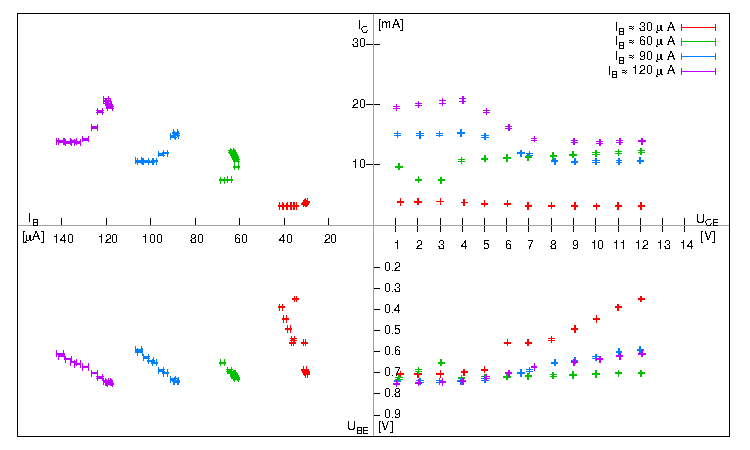
\includegraphics[width=20cm]{graphen/curve0}}
\captionof{figure}{Gemessenes Kennlinienfeld}%
\label{gnuplot_kennlinienfeld}
\end{minipage}
\end{center}